\subsection{Růst a pokles funkce}
O funkci řekneme, že je \begin{itemize}
    \item \textbf{rostoucí} na intervalu $I$, jestliže pro všechna $x,y \in I$ splňující $x<y$ platí $f(x) < f(y)$,
    \item \textbf{klesající} na intervalu $I$, jestliže pro všechna $x,y \in I$ splňující $x<y$ platí $f(x) < f(y)$,
    \item \textbf{neklesající} na intervalu $I$, jestliže pro všechna $x,y \in I$ splňující $x<y$ platí $f(x) \leq f(y)$,
    \item \textbf{nerostoucí} na intervalu $I$, jestliže pro všechna $x,y \in I$ splňující $x<y$ platí $f(x) \geq f(y)$,
    \item \textbf{monotónní} na intervalu $I$, jestliže je na něm neklesající, anebo nerostoucí,
    \item \textbf{konstantní} na intervalu $I$, jestliže pro všechna $x,y \in I$ splňující $x<y$ platí $f(x) = f(y)$.
\end{itemize}

\begin{figure}[H]
    \centering
    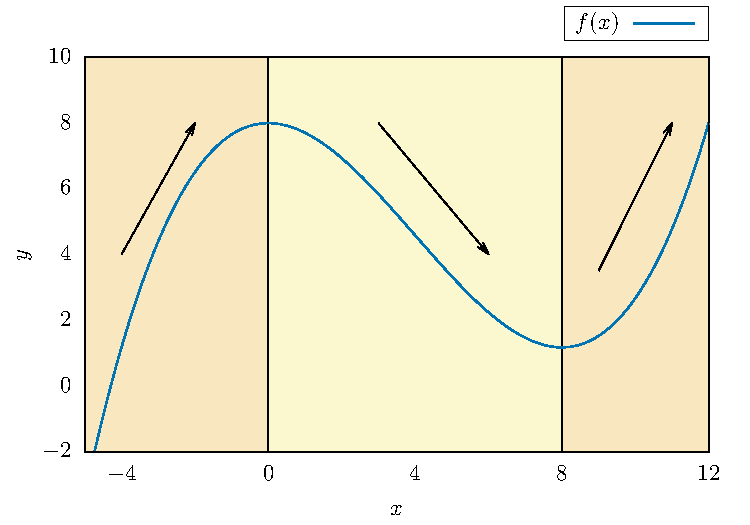
\includegraphics[scale = 0.7]{Gnuplot/Figures/funkce-rostouci-klesajici-obr.pdf}
    \caption{Ilustrace pojmu rostoucí a klesající funkce. Na oranžové oblasti je $f(x)$ rostoucí, na žluté oblasti je $f(x)$ klesající.}
\end{figure}

\begin{remark}
    Pokud mluvíme o růstu nebo poklesu funkce, je vždy nutné uvést, na jakém intervalu se pohybujeme. Důležitost je vidět na následujícím příkladu, viz obrázek \ref{fig:1a-funkce-ne}.

    \begin{figure}[H]
        \centering
        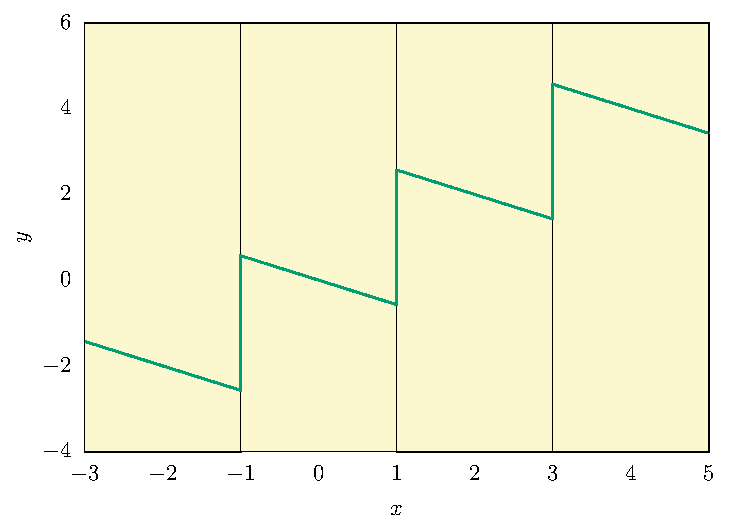
\includegraphics[scale = 0.7]{Gnuplot/Figures/periodicka-klesajici.pdf}
        
        \caption{Příklad funkce, která je klesající na každém intervalu $I_p = (2p-1,2p+1)$, kde $p \in \Z$. Na celém $\R$ ale není ani rostoucí, ani klesající. Porovnáme-li dva body $x_1 < x_2$ v témže intervalu $I_p$, splňují $f(x_1) > f(x_2)$. Porovnáme-li však body v různých intervalech, dostaneme $f(x_1) < f(x_2)$. Není tedy splněna ani jedna z podmínek pro růst nebo pokles na $\R$. Všimněme si, že funkce je v krajních bodech intervalů nespojitá, má v nich skoky.}
        \label{fig:1a-funkce-ne}
    \end{figure}

\end{remark}

\begin{remark}
    V některé literatuře se o různých křivkách mluví jako o \uv{rostoucích zleva doprava} nebo \uv{klesajících zprava doleva} a podobně. Matematická terminologie vždy pracuje s tím, co se děje s hodnotami $f(x)$ \underline{při rostoucích $x$} - tedy vždy \uv{zleva doprava}, chcete-li. Podobně se někdy říká o klesajících funkcích $y(x)$, že \uv{$y$ je nepřímo úměrné $x$}. Ale matematická terminologie říká, že pouze funkce $y(x)=C/x$ je nepřímá úměrnost, žádná jiná funkce toto nesplňuje.

    \begin{figure}[H]
        \centering
        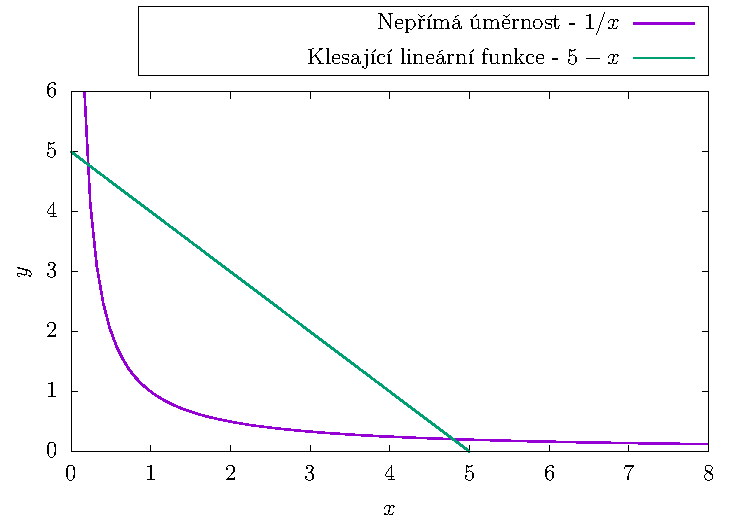
\includegraphics[scale = 0.7]{Gnuplot/Figures/neprima-umernost.pdf}
        \caption{Ilustrace často nesprávně použitého termínu \uv{nepřímá úměrnost}. Pouze funkce typu $C/x$ jsou nepřímé úměrnosti.}
    \end{figure}
\end{remark}

\subsection{Další charakteristiky funkce}

O funkci $f(x)$ říkáme, že je \begin{itemize}
    \item \textbf{prostá} na intervalu $I$, jestliže pro všechna $x,y \in I$ splňující $x \neq y$ platí $f(x) \neq f(y)$ (\uv{každému $x$ přísluší jiná hodnota $f(x)$}),
    \item \textbf{omezená shora}, jestliže existuje konečné číslo $K$ takové, že pro všechna $x \in D(f)$ platí $f(x) \leq K$,
    \item \textbf{omezená zdola}, jestliže existuje konečné číslo $K$ takové, že pro všechna $x \in D(f)$ platí $f(x) \geq K$,
    \item \textbf{omezená}, jestliže je omezená shora i zdola.
\end{itemize}